\section{质量}\label{sec:1-5}

空气、水、铜、铁、木材、胶等都是物质,所有的物体,比如桌子、椅子、飞机、轮船都是由物质组成的。
物体里所含的物质有多有少,一桶水比一杯水所含的水多,大铁块比小铁棒所含的铁多。
为了说明物质的多少,物理学里引入了\textbf{质量}这个物理量。

\textbf{物体所含物质的多少叫做质量}。

把一块铁轧成铁片,形状变了,但所含铁的多少没有变。也就是质量没有变。
一块冰融化成水,由固体变成了液体,物质的状态变了,但所含水的多少没有变,质量也就没有变。
可见,\CJKunderwave{质量是物体本身的一种属性},它不随物体的形状、温度、状态而改变。
质量也不随物体的位置而改变。
一罐头水果,不论把它放在赤道还是北极,罐头里水果的多少都不会改变,所以质量也不会改变;
就是被宇航员带到月球上,质量也不会改变。


\begin{wrapfigure}[13]{r}{7cm}
    \centering
    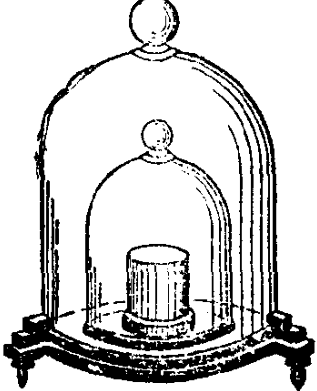
\includegraphics[width=0.2\textwidth]{../pic/czwl1-ch1-13}
    \caption{国际千克原器}\label{fig:1-13}
\end{wrapfigure}


在日常生活中,人们经常要测量物质的质量。
比如我们买柴、买米,总要用秤称一称,称的就是柴和米的质量。
在科学技术中也要经常测量质量。

为了测量物体的质量,需要定出质量的单位。在国际单位制里,质量的主单位是\textbf{千克}(也叫公斤)。
原来人们规定在 $4\celsius$ 时 1 升纯水的质量为 1 千克。
后来根据这个规定,用铂铱合金制成一个质量是 1 千克的圆柱体,作为 1 千克的标准,叫做国际千克原器(图 \ref{fig:1-13}),保存在法国巴黎的国际计量局里。
为了测量质量很小的物体,还规定了比千克小的单位——克和毫克,
\vspace{-1em}\begin{center}
    \begin{tabular}{l}
        1 千克 = 1000 克, \\
        1  克 = 1000 毫克。 \\
    \end{tabular}
\end{center}\vspace{-1em}
测量质量较大的物体时,通用用吨作为单位,

\centerline{1  吨 = 1000 千克。}

\begin{table}[H]
    \centering
    \caption*{\textbf{一些物体的质量} (单位:千克)}
    \begin{tabular}{w{l}{10em}w{r}{8em}}
        银河系      & $2.8 \times 10^{41}$ \\
        太阳        & $2.0 \times 10^{30}$ \\
        地球        & $6.0 \times 10^{24}$ \\
        月球        & $7.4 \times 10^{22}$ \\
        尘埃微粒    & $6.7 \times 10^{-10}$ \\
        青霉素分子  & $5.0 \times 10^{-17}$ \\
        氢原子      & $1.7 \times 10^{-27}$ \\
        电子        & $9.1 \times 10^{-31}$ \\
    \end{tabular}
\end{table}

\,
